%%=====================================================================
%% METODOLOGIA (TCC, cap. 3): planejamento, sistema, placa, sensor,
%% supervisório, identificação, ajuste dos ganhos, ensaio da hélice
%%=====================================================================
\secaoudesc{Metodologia}

\begin{frame}{Planejamento}
  \centering
  \tikzfig{1}{0.55}{plan_janelas}
  \vspace{0.6em}
  \begin{itemize}
    \item Três frentes em paralelo: mecânica (CAD), placa de medição e
          interface
    \item Cada etapa validada em simulação antes do \textit{hardware}
  \end{itemize}
  \fonte
\end{frame}

\begin{frame}{Planejamento: CAD}
  \centering
  \tikzfig{1}{0.8}{plan_cad}
  \fonte
\end{frame}

\begin{frame}{Planejamento: placa de medição}
  \centering
  \tikzfig{1}{0.8}{plan_placa}
  \fonte
\end{frame}

\begin{frame}{Planejamento: interface de usuário}
  \centering
  \tikzfig{1}{0.8}{plan_interface}
  \fonte
\end{frame}

\begin{frame}{Arquitetura do sistema de aquisição}
  \centering
  \tikzfig{1}{0.68}{arq_comunicacao}
  \fonte[Autor (2026); An (2026)]
\end{frame}

\begin{frame}{Cadeia de aquisição}
  \centering
  \tikzfig{1}{0.78}{blocos_aquisicao}
  \fonte
\end{frame}

\begin{frame}{Gabinete: potência e segurança}
  \centering
  \tikzfig{1}{0.8}{gabinete}
  \fonte
\end{frame}

\begin{frame}{Placa de medição: camadas do \textit{firmware}}
  \centering
  \tikzfig{1}{0.7}{fw_camadas}
  \fonte[Autor (2026); Zephyr Project (2026)]
\end{frame}

\begin{frame}{Escolha do sensor de corrente}
  \centering
  \tikzfig{0.95}{0.42}{escolha_sensor}
  \vspace{0.8em}
  \begin{itemize}
    \item Requisitos: isolação galvânica, resposta em corrente contínua,
          baixo custo por fase
    \item Escolha: núcleo toroidal concentrador com sensor Hall SS49E
  \end{itemize}
  \fonte[Autor (2026); Ziegler et al.\ (2009)]
\end{frame}

\begin{frame}{Sensor Hall com núcleo toroidal}
  \centering
  \tikzfig{1}{0.72}{sensor_topologia}
  \fonte[Autor (2026); Honeywell International Inc.\ (2016)]
\end{frame}

\begin{frame}{Ensaio de caracterização do conjunto núcleo--sensor}
  \centering
  \tikzfig{1}{0.8}{sensor_ensaio}
  \fonte
\end{frame}

\begin{frame}{Placa de condicionamento das fases (AQ1)}
  \centering
  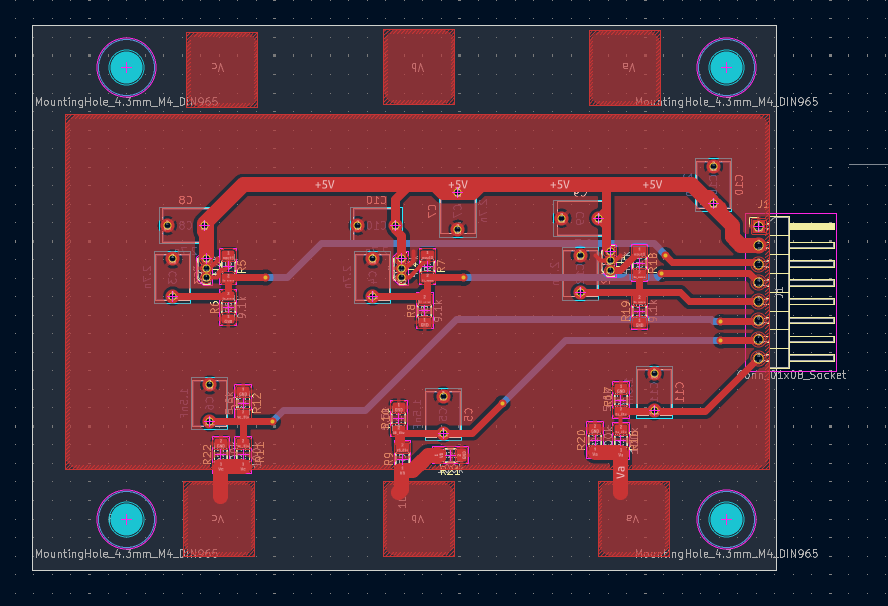
\includegraphics[width=\linewidth,height=0.72\textheight,keepaspectratio]{Metodologia/placa aq1 SAME.png}
  \fonte
\end{frame}

\begin{frame}{Observador embarcado}
  \centering
  \tikzfig{1}{0.66}{smo_hibrido}
  \begin{itemize}
    \small
    \item SMO estima a FEM; PLL extrai ângulo e rotação
    \item Torque: correntes \emph{medidas} projetadas no ângulo estimado
  \end{itemize}
  \fonte[Adaptado de Utkin (1992); Kaf et al.\ (2024)]
\end{frame}

\begin{frame}{Aplicação de supervisão}
  \centering
  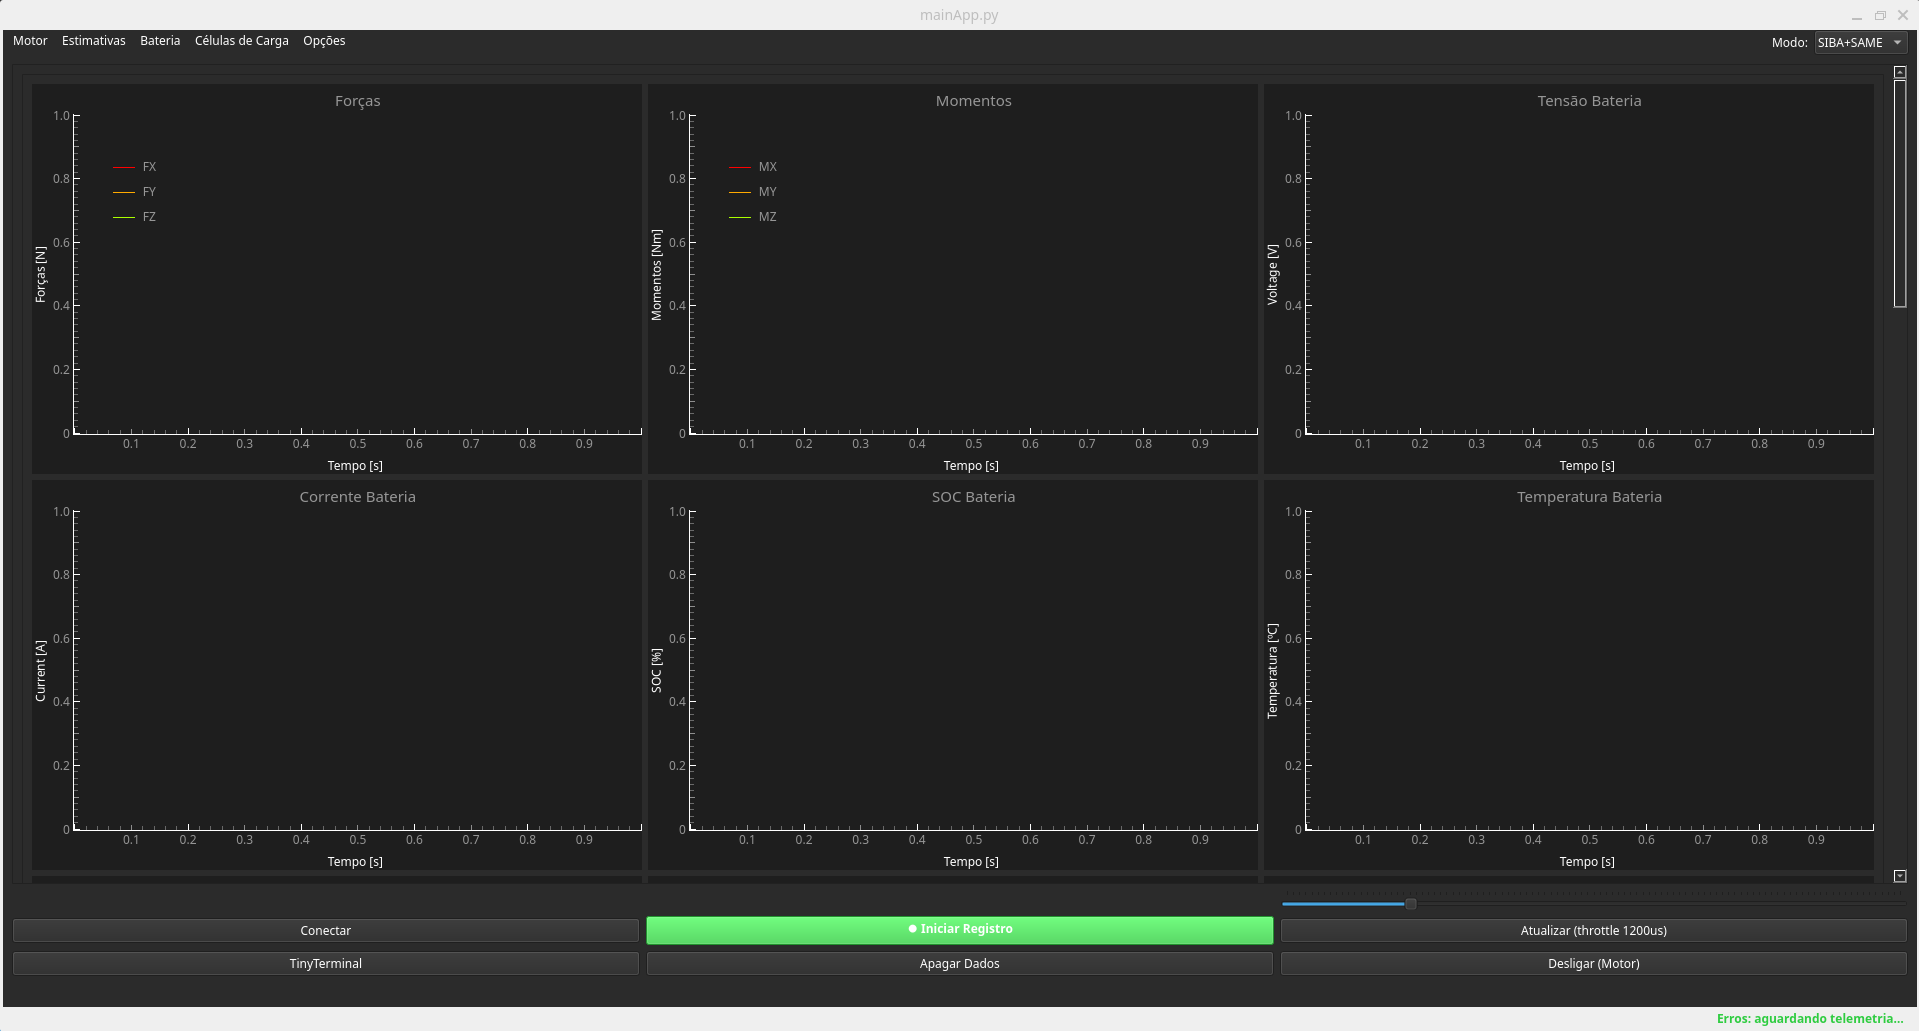
\includegraphics[width=\linewidth,height=0.72\textheight,keepaspectratio]{Metodologia/gui tela principal.png}
  \fonte
\end{frame}

\begin{frame}{Protocolo em arquivo único}
  \centering
  \tikzfig{1}{0.72}{yaml_fluxo}
  \fonte
\end{frame}

\begin{frame}{Identificação dos parâmetros do motor}
  \begin{columns}[c]
    \begin{column}{0.45\textwidth}
      \begin{itemize}
        \small
        \item Resistência: quatro terminais (Kelvin)
        \item Indutância: ressonância $LC$ e ajuste harmônico aos registros
              em rotação
        \item Perdas a vazio: patamares de rotação, $T_{perdas} = B\,\omega
              + \tau_c$
        \item Registros com osciloscópio, tacômetro óptico e neutro virtual
      \end{itemize}
    \end{column}
    \begin{column}{0.55\textwidth}
      \centering
      \tikzfig{1}{0.68}{motor_rotor_bloqueado}
      \fonte[Autor (2026); Fitzgerald, Kingsley e Umans (2014)]
    \end{column}
  \end{columns}
\end{frame}

\begin{frame}{Ajuste automático dos ganhos do observador}
  \[
    J(\mathbf{x}) = \frac{1}{M}\sum_{q=1}^{M}
      \Big( w_T\,g_{T,q} + w_\omega\,g_{\omega,q}\Big),
    \qquad w_T = 1{,}0,\; w_\omega = 0{,}5
  \]
  \centering
  \tikzfig{1}{0.55}{fluxo_autotune}
  \fonte[Autor (2026); Storn e Price (1997)]
\end{frame}

\begin{frame}{Ensaio do coeficiente de torque da hélice}
  \centering
  \tikzfig{1}{0.4}{fluxo_helice}
  \[
    Q = \hat{T}_e - (B\,\omega + \tau_c), \qquad
    C_Q = \frac{Q}{\rho\,n^2 D^5}
  \]
  \begin{itemize}
    \small
    \item Patamares de acelerador; média de rotação e torque em regime
    \item Referência: curva APC na condição estática
  \end{itemize}
  \fonte[Autor (2026); APC Propellers (2026)]
\end{frame}
